\section{System Overview}
As stated in the requirements, the system should handle stremaing video from a camera, perform convolution and be able to provide the result as an ouput stream.
The convolution is to be done on the FPGA using a custom processor implementation described in section \ref{sec:processor}.
To make the FPGA as simple as possible, the campera is connected to and controlled by the EFM, and the video is passed to the convolution processor in a suitable format.

Furthermore, as HDMI output is not available on the EFM and the bus between the EFM and FPGA is already assumed to be a bottleneck, the HDMI output is placed on the FPGA.

Figure \ref{fig:systemArchitecture} displays the overall system architecture. Notice how data flows from left to right.

\begin{figure}[h!]
    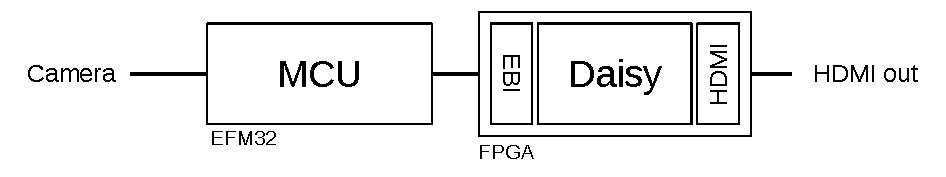
\includegraphics[]{img/systemArchitecture.pdf}
    \caption{System Architecture}
    \label{fig:systemArchitecture}
\end{figure}

During the project, a risk assessment was done to find and reduce the risk of failure.
Some of the measures taken was to add an extra HDMI port connected to the FPGA in case we failed to transfer video from the EFM to the FPGA.
